% !TEX root = ../distCjHMSC.tex
%================================
The results of this section report the estimation for the eight locations given in the table \ref{tab:sensor-specifications}.

%================================
%================================
\section{General pipeline for the estimation process}
%================================
The general pipeline proposed for the estimation process is reported figure \ref{fig:pipeline}. It consists 
\begin{itemize}
\item
of a filter bank described in a file of settings which is characterized by a sequence of following descriptors: type, frequency lower bound, upper frequency bound, order, desired stationarity duration etc. Commonly used type is Butterworth (available on Matlab).
\item
At the output of a filter, the two signals (one for the SUT the other for the SREF) are shared in non-overlapping blocks to perform the spectral estimate. Longer the size of a block more accurate the spectral analysis. But that assumes stationarity, and the real signals do not exhibit permanent stationarity. Therefore we can choose in the setting file the desired stationarity duration in term of multiple of the longest period in the band (inverse of lower frequency bound). Typically we take  $5$ times the longest period, expecting that we can find such length with stationarity to estimate the spectral components. Even with that, the accuracy is not in accordance with the PTS requirements, but by averaging in a long period of times (many days), we can reach such requirements.


\item
Each block is then shared in overlapping sub-blocks. We can choose the windowing and the overlap rate. Typically we consider Hann windowing and $50\%$ of overlapping. The periodograms in the different sub-blocks are averaged to provide a spectral estimation. 

Only estimates in the bandwidth of the filter are retained.

\item
MSC is performed in each bandwidth. If the MSC is above the selected threshold, the value of the ratio $\hat S_{UU,k}/\hat S_{RU,k}$ is saved.



\item
along the recorded data, for a given frequency index $k$, the values  $\hat S_{UU,k}/\hat S_{RU,k}$ are averaged with weighting factors in accordance with $\hMSC$ values.


\item
Finally the estimation of the SUT response is derived from the SREF response.


\end{itemize}

%=================================
\subsubsection{Filter bank analysis}
%=================================
Let us recall that in a first step, the signals are filtered in adjacent bands in such a way to use different periods whose the main interest is to consider short periods, if necessary, in the high frequency bands. The table \ref{tab:freq-duration-tradeoff} is an example of pavement, consisting of $5$ bands with log-spaced filter parameters in the band $(0.01-5)$ Hz with a variable window length\footnote{See also recent PMCC reports.}. Because the two signals are applied to the same filter we can use RII as Butterworth filter. Also because this process is for anlysis, we don't need to downsampling and/or to require perfect recontruction. Even more the bandpass filters can be overlap in the frequency domain. Although a decimation can be used to save computational time, indeed the bandwidths are lower than $F_{s}/2$, that operation is not considering in the following.

\begin{table}
\begin{center}
\begin{tabular}{|c|c|}
\hline
frequency band (Hz) & stationarity period (second)
\\
\hline
%%%%% from matlab
$[0.02-0.20]$&$400$
\\ \hline $[0.20-1.00]$&$200$
\\ \hline $[1.00-2.00]$&$100$
\\ \hline $[2.00-3.00]$&$50$
\\ \hline $[3.00-4.00]$&$25$
\\ \hline $[4.00-6.00]$&$25$
\\ \hline 
%%%%
\end{tabular}
\parbox{12 cm}
{
    \caption{\protect\small\it  }
    \label{tab:freq-duration-tradeoff}
}
\end{center}
\end{table}
\figscale{filterbank.pdf}{Filter bank}{fig:filterbank}{1}


%================================
\newpage\clearpage
%================================
%================================section{Numerical results}
%================================

%================================
\subsection{Results of IS26}
%================================
In this section we report analysis of the data from IS2. The numerical values are reported in figures from \ref{fig:C2} to \ref{fig:C8} associated with the sensors 1 to 8.

 \figscale{afewdaysonI26C1H1.pdf}{Couple H1C1}{fig:C1}{1}
 
 \figscale{afewdaysonI26C2H2.pdf}{Couple H2C2}{fig:C2}{1}
  \figscale{afewdaysonI26C3H3.pdf}{Couple H3C3}{fig:C3}{1}

 \newpage
 \figscale{afewdaysonI26C4H4.pdf}{Couple H4C4}{fig:C4}{1}
 \figscale{afewdaysonI26C5H5.pdf}{Couple H5C5}{fig:C5}{1}

 \newpage
 \figscale{afewdaysonI26C6H6.pdf}{Couple H6C6}{fig:C6}{1}
 \figscale{afewdaysonI26C7H7.pdf}{Couple H7C7}{fig:C7}{1}

 \newpage
  \figscale{afewdaysonI26C8H8.pdf}{Couple H8C8}{fig:C8}{1}



%================================
\newpage\clearpage
%================================
%================================
\section{More comments}
%================================
\subsection{Effect of the selected MSC}
%================================
We said that we can not choose a too low value for the MSC threshold because the underdetermination. That appears clearly on figure \ref{fig:afewdaysonI26C6H6twoMSC}.
When the  MSC threshold is $0.7$, there is a large discrepancy between the estimated ratios, see \eqref{eq:estimated-Ratio} and we outline that there is no way to solve the underdetermination. But for an MSC threshold of $0.95$, the two curves are very close.

\figscale{afewdaysonI26C6H6twoMSC.pdf}{Couple H6C6, for two MSC thresholds.}{fig:afewdaysonI26C6H6twoMSC}{0.7}

On the other hand if the ratio between the two noise levels are perfectly known the indetermination is removed and we can use formula \eqref{eq:known-noise-ratio}. You might be tempted to say that the two noises on the two sensors are identical except theirs levels and consider that the ratio is given by the number of inlets in the noise reduction system. However the figure \ref{fig:afewdaysonI26C4H4knownnoiseratio} shows that the curve with a MSC threshold of $0.5$ and the formula \eqref{eq:known-noise-ratio} lead to values different from the curves obtained with a a MSC threshold of $0.95$.

\figscale{afewdaysonI26C4H4knownnoiseratio.pdf}{Couple H4C4, for two MSC thresholds with formula \eqref{eq:known-noise-ratio}.}{fig:afewdaysonI26C4H4knownnoiseratio}{0.7}

%================================
\newpage\clearpage
%================================
\subsection{Dip on the curves}
%================================
For the figures \ref{fig:C2} to \ref{fig:C5} associated to the MB2005, an important dip around 0.1 Hz is observed. 

Also we have reported figure \ref{fig:afewdays1colocation} a few days on the location H2C2. The different colors are for different days. The distribution seems to be uniform and does not depend on the day. The ratio seems to be different of 1.\\*

If the MSC is about 0.99, meaning that the noises on the two sensors are negligible, and if the two sensors have the same response, the only reason to get a ratio less than 1, is that the acoustical SOI on the SUT is attenuated, may due to the noise system reduction. That would write: it exists $\alpha\in\mathbb{C}$ with $|\alpha|<1$ s.t.:
\begin{eqnarray}
\label{eq:model-of-obervation}
\left\{
\renewcommand\arraystretch{1.6}
\begin{array}{rcl}
x_{\ut}(t)&=&g_{\ut}  \star (\alpha s(t))
\\
x_{\rf}(t)&=&g_{\rf}  \star s(t)
\end{array}
\right.
\end{eqnarray}

\figscale{afewdays1colocation.pdf}{a few days on H2C2. Only the band $[0.08-0.12]$ Hz is selected. The coherence is above $0.99$. The different colors for the different days.}{fig:afewdays1colocation}{0.5}


Another way to see the response differences between the 2 sensors in the band  $[0.08-0.12]$ Hz (gain ratio different of 1), appears figure \ref{fig:filteredsignals}. A zoom of the signals is plotted. It consists of about 1 minute, around a position where the observed coherence is above $0.99$. We see that the signal on the SREF  is bigger than this on the SUT. There is no way and no reason to reject this time window since the difference can be due either to the loss of gain or a unknown transfer function. 
\begin{figure}%{20cm}
\begin{minipage}{10cm}
              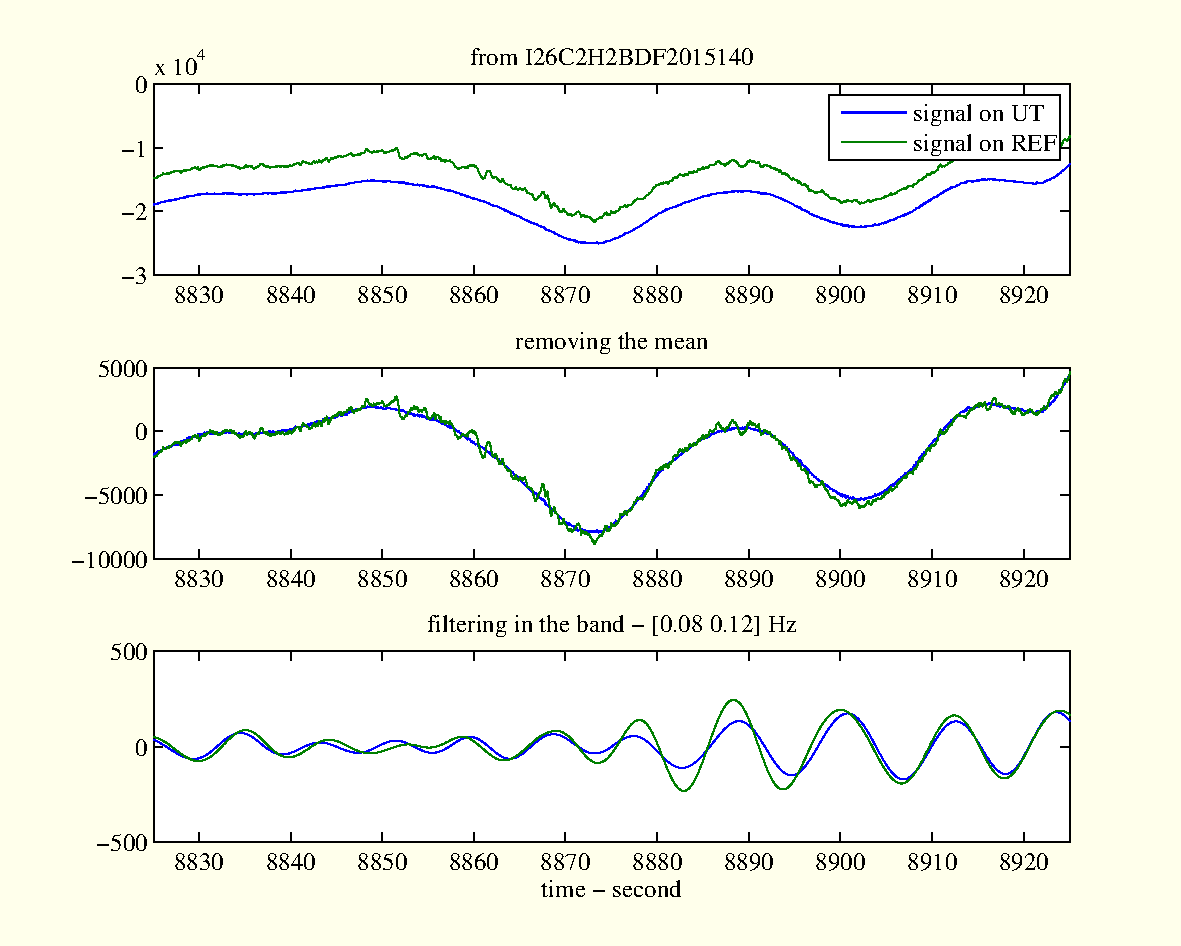
\includegraphics[scale=0.5]{signalsanomaly.pdf}
\end{minipage}
\begin{minipage}[c]{8cm}
              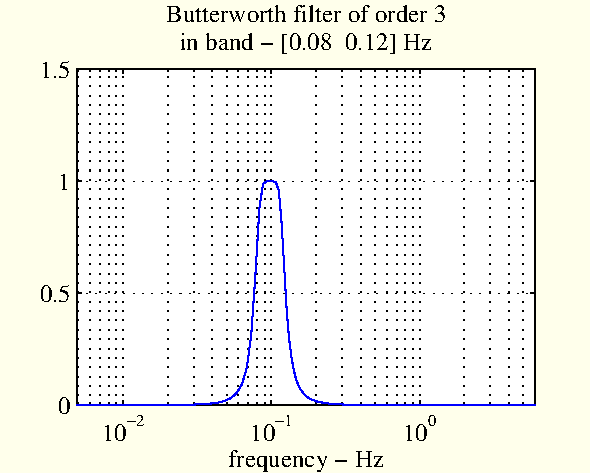
\includegraphics[scale=0.5]{filteranomaly.pdf}    

\end{minipage}
\centering
\caption{Filtered signals}
\label{fig:filteredsignals}
\end{figure}

